\documentclass[11pt]{article}
	\usepackage[T1]{fontenc}
	\usepackage[english]{babel}
	\usepackage[utf8]{inputenc}
	\usepackage{graphicx}
	\usepackage{float}
	\usepackage{amsfonts, amsmath}
	\usepackage{fancyhdr}
	\usepackage{setspace}
	\usepackage{epstopdf}
	\usepackage{listings}
	\usepackage{color}
	\usepackage{xspace}
	\usepackage{multirow}
	\usepackage{caption}
	
	\newcommand{\latex}{\LaTeX\xspace}
	\graphicspath{images}
	
	\pagestyle{fancy}
	\fancyhead{}
	\fancyfoot{}
	\fancyfoot[R]{\thepage}
	
	\textheight 21.0cm
	\topmargin -0.5cm
	
	\setlength{\parindent}{0ex}
	\setlength{\parskip}{1em}

	\definecolor{mygreen}{rgb}{0,0.6,0}
	\definecolor{mygray}{rgb}{0.5,0.5,0.5}
	\definecolor{mymauve}{rgb}{0.58,0,0.82}

\lstset{ %
  backgroundcolor=\color{white},   % choose the background color; you must add \usepackage{color}
  basicstyle=\footnotesize,        % the size of the fonts that are used for the code
  breaklines=false,                 % sets automatic line breaking
  commentstyle=\color{mygreen},    % comment style
  frame=single,	                   % adds a frame around the code
  keepspaces=true,                 % keeps spaces in text, useful for keeping indentation of code (possibly needs columns=flexible)
  language=C++,                 % the language of the code
  numbers=left,                    % where to put the line-numbers; possible values are (none, left, right)
  numbersep=5pt,                   % how far the line-numbers are from the code
  numberstyle=\tiny\color{mygray}, % the style that is used for the line-numbers
  stepnumber=1,                    % the step between two line-numbers. If it's 1, each line will be numbered
  stringstyle=\color{mymauve},     % string literal style
  tabsize=2,	                   	 % sets default tabsize to 2 spaces
  title=\lstname                   % show the filename of files included with \lstinputlisting; also try caption instead of title
}

\renewcommand{\headrulewidth}{0pt}
			
\begin{document}
\setstretch{1.0}
\renewcommand*\contentsname{Table of contents}
	%\begin{titlepage}
	\begin{center}
		\begin{tabular}{| c | c |}
		\hline
		Wroclaw University of Technology & Dr Ewa Szlachcic\\ \hline
		Faculty of electronics & Optimization Theory and
		Numerical Methods \\
		Control Engineering and Robotics & Project - AREU0003\\
		$2^{nd}$ cycle studies & \\ \hline
		\multicolumn{2}{c}{Non-linear programming for multicriterial problems}\\
			\hline
	\end{tabular}			
	\end{center}
	
	\textbf{Topic:} Bicriterial optimization of non-linear functions with
	constraints - Niched Pareto Genetic Algorithm (NPGA).
	
	\begin{center}
		\begin{tabular}{| l | c |}
		\hline
		Authors & Tomasz Bartos, 209248\\
				& Radoslaw Zwolski, 209124\\ \hline
		Project group & Monday, 13:15-15:15, Odd weeks\\ \hline
		Project due date & 22.05.2017\\
		\hline
	\end{tabular}
	\end{center}
	
	\newpage
	
	\tableofcontents
	
	\newpage

	\section{Introduction}
	
	The aim of the project was to implement an optimization algorithm of non-linear
	bicriterial problem. Niched-Pareto Genetic Algorithm (NPGA) has been used to
	solve this problem. Whole program has been implemented in C++ using QT 	
	framework and allows user to provide functions to optimize as well 
	as configuration parameters by GUI (Graphical User Interface). The result of 
	algorith has been shown as Pareto chart and table of non-dominated points.
	
	\section{Description of the problem}
	
	\subsection{Definition of problem}
		
	The algorithm solves a bicriterial problem. Here it minimizes system of two
	functions with M variables.
	
	$$\begin{cases}
		f_{1}(x_{1},x_{2},...,x_{M})\\
		f_{2}(x_{1},x_{2},...,x_{M})
	\end{cases}$$
	
	These functions can be either linear or nonlinear. Constraints given as an
	input of the algorithm are constraints of variables. So:
	
	$$\begin{cases}
		x_{1min} \leq x_{1} \leq x_{1max}\\
		x_{2min} \leq x_{2} \leq x_{2max}\\
		.\\
		.\\
		.\\
		x_{Mmin} \leq x_{M} \leq x_{Mmax}\\
	\end{cases}$$
	
	
	\begin{figure}[H]
	\caption{The idea of pareto optimal points selected from set of feasible
	points}
	\centering
	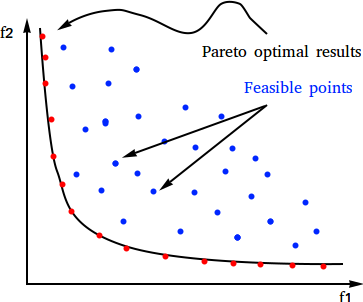
\includegraphics[scale=0.8]{pareto_definition}
	\label{fig:pareto_idea}
	\end{figure}
	
	\begin{figure}[H]
	\caption{The idea of pareto optimal points selected from set of feasible
	points}
	\centering
	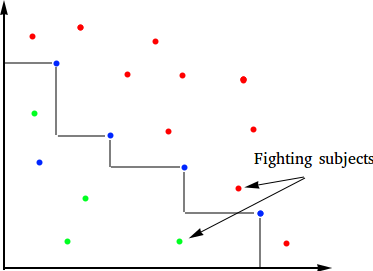
\includegraphics[scale=0.8]{comparative_set}
	\label{fig:pareto_idea}
	\end{figure}
	
	
	\begin{figure}[H]
	\caption{Application window view}
	\centering
	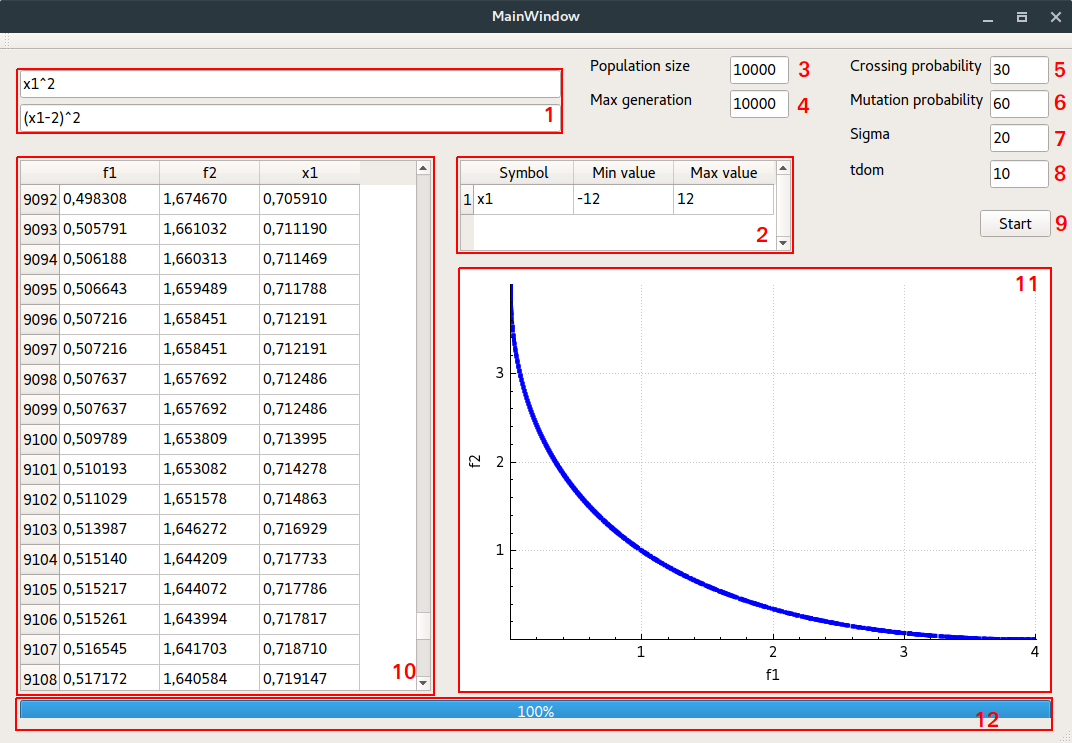
\includegraphics[scale=0.35]{application}
	\label{fig:app_window}
	\end{figure}
	
	\begin{enumerate}
		\item Boxes in which user should write two functions for finding pareto
			optimal points. Top box will then be recognized as $f_{1}$ when the 
			bottom box will be recognized as $f_{2}$
		\item Table that will represent list of variables recognized in functions
			formulas that should be inserted before. Here a user can define 
			constraints of those variables writing them in "Min" and "Max" columns.
		\item Population size $N$ - amount of points that will be generated as
			($f_{1}$, $f_{2}$)
		\item Maximum generation $t$ - amount of repeats of whole algorithm
		\item Crossing probability $p_{c}$ - probability of performing crossing
			operation on a particular point.
		\item Mutation probability $p_{m}$ - probability of performing mutating
			operation on a particular point
		\item Sigma $\sigma$ - is a parameter that specifies radius of niche. It is
			distance of a chosen point 
		\item Amount of points in comparative collection $t_{dom}$
		\item Start button - clicking on it triggers start of calculations, if
			functions have been specified as well as all of parameters needed and
			described in points 1-8. If user will click on Start button before
			specifying a particular parameter it will have $0$ value by default.
		\item Table consisting points of pareto - table consisting pareto optimal
			points with value of $f_{1}$ and $f_{2}$ as well as values of every
			variable that resulted in generating such values of given functions
		\item Figure - figure showing pareto optimal points on a plot with
			coordinate system axis set as: axis of absenteeism being values of
			$f_{1}$ and axis of ordinates being values of $f_{2}$
		\item Progress bar showing progress of a testcase run to keep user in
			knowledge of progress of the calculations.
			
		\begin{center}
		\captionof{table}{Fields possible to fill by a user and their acceptable 
			values}
		\begin{tabular}{| c | c | c |}
			\hline
			Data field & Data type & Possible values\\ \hline
			Function & string & Attachment A\\ \hline
			Variable & string & x1, x2, ..., xm \\ \hline
			Min constraint & real number & $-1.7e+308 \div 1.7e+308$\\ \hline
			Max constraint & real number & $-1.7e+308 \div 1.7e+308$\\ \hline
			Population size $N$ & natural number & $0 \div 2^{31}-1$ \\ \hline
			Max generations $t$ & natural number & $0 \div 2^{31}-1$ \\ \hline
			Crossing probability & natural number & $0 \div 100$ \\ \hline
			Mutation probability & natural number & $0 \div 100$ \\ \hline
			$\sigma$ & real number & $0 \div 1.7e+308$ \\ \hline
			$t_{dom}$ & natural number & $0 \div 2^{31}-1$, $t_{dom} \leq N$ \\
			\hline
		\end{tabular}			
		\end{center}
			
	\end{enumerate}
	
\end{document}